\documentclass[11pt]{beamer}

% Theme and Color Customization
\usetheme{Madrid}
\definecolor{mygreen}{RGB}{0, 153, 76}
\usecolortheme[named=mygreen]{structure}
\useinnertheme{rounded}
\useoutertheme{miniframes}

% Packages
\usepackage{graphicx}
\usepackage{bm}
\usepackage{booktabs}
\usepackage{amsmath, amssymb}
\usepackage{tikz}
\usepackage{listings}
\usepackage{xcolor}
\usepackage{hyperref}
\usepackage[backend=biber,style=numeric,sorting=none]{biblatex}
\newcommand{\stb}{\mathcal{U}_{\text{STB}}}
\usepackage{amsmath, amsthm}
% Enable theorem-like environments in Beamer
\setbeamertemplate{theorems}[numbered]

% Define a new lemma environment with numbering
\newtheorem{customlemma}{Lemma}
\newtheorem{customobservation}{Observation}

% Add bibliography file
\addbibresource{references.bib}

% Code Listings Style
\lstset{
  basicstyle=\ttfamily\small,
  keywordstyle=\color{blue}\bfseries,
  commentstyle=\color{gray},
  stringstyle=\color{orange},
  showstringspaces=false,
  breaklines=true,
  frame=single,
  backgroundcolor=\color{black!5}
}

% Title page details
\title[Robust Two-Stage RTP]{Robust Two-Stage Radiotherapy Treatment Planning}
\author[Jonathan Wolloch]{Jonathan Wolloch\\Advisor: Dr. Shimrit Shtern}
\institute[Technion]{Faculty of Data and Decision Sciences\\Technion - Israel Institute of Technology}
\date{\today}

% Document
\begin{document}

% Title Slide
\begin{frame}[plain]
  \titlepage
\end{frame}

% Outline
\begin{frame}{Outline}
  \tableofcontents
\end{frame}

% Section 1
\begin{frame}{Outline}
  \begin{itemize}
    \item Handling Uncertain Data With Robust Optimization
    \item Optimizing Radiotherapy Treatment Planning
    \item Numerical Experiments
    \item Future Directions
  \end{itemize}
\end{frame}

% Section 2
\section{Handling Uncertain Data With Robust Optimization}
\begin{frame}{Handling Uncertain Data With Robust Optimization}
  \begin{enumerate}
    \setlength{\itemsep}{1em}
    \item We would like to assume that good data leads to good decisions.
    \item However, as reported in \cite{ben-tal2000}, for some LPs even a 0.01\% perturbation in the data may cause certain constraints to become highly infeasible.
  \end{enumerate}
\end{frame}

\begin{frame}{Several Key Observations}
    \begin{enumerate}
        \setlength{\itemsep}{1em}
      \item At the time of decision making, data isn't known exactly.
      \item We cannot ignore this uncertainty.
      \item A methodology for handling this uncertainty is needed.
    \end{enumerate}
  \end{frame}

  \begin{frame}{Enter Robust Optimization (For the LP case)}
A generic LP can be characterized with the triplet $(A, b, c)$.
      \[
        \min_{x \in \mathbb{R}^n} \{c^T x : Ax \leq b\}
      \]
In the robust optimization framework, an \textit{uncertain-LP} is defined as a collection:
      \[
        \min_{x \in \mathbb{R}^n} \{c^T x : Ax \leq b, \forall (A, b, c) \in \mathcal{U}\}
      \]
What does it mean to solve an uncertain-LP?
  \end{frame}
  

% Math Example
\begin{frame}{The Underlying Decision-Making Environment}
  \begin{enumerate}
    \setlength{\itemsep}{1em}
    \item $x$ represents "here-and-now" decisions.
    \item The decision-maker is fully responsible for the consequences of the decisions, only when the actual data is within $\mathcal{U}$.
    \item The decision-maker cannot tolerate violations of the constraints when the data is in $\mathcal{U}$.
  \end{enumerate}
\end{frame}

\begin{frame}{An "uncertainty immunized" solution}
      In this environment, an uncertainy immunized solution is a fixed vector that remains feasible whatever the realization of the data within $\mathcal{U}$.\\
      \vspace{1em}
      We call such a solution \textit{robust feasible}.
  \end{frame}

\begin{frame}{What is the value of a \textit{robust feasible} solution?}
    Since we want a solution that is feasible no matter the realization, it is natural to attribute the worst-case value of the uncertain-LP to the robust feasible solution, that is:
    \[
    \sup\{c^T x : (A, b, c) \in \mathcal{U}\}
    \]
    Thus, the best \textit{robust feasible} solution can be found by solving the following LP:
    \[
    \min_{x} \{\sup_{(A, b, c) \in \mathcal{U}} c^T x : Ax \leq b,\; \forall (A, b, c) \in \mathcal{U}\}
    \]
    or equivalently:
    \[
    \min_{x, t} \{t : c^T x\le t,\; Ax \leq b,\; \forall (A, b, c) \in \mathcal{U}\}
    \]
\end{frame}

% Section 3
\section{Optimizing Radiotherapy Treatment Planning}
\begin{frame}{Discovery of X-rays}
In 1895, Wilhelm Conrad Röntgen documented his discovery of X-rays, earning him the Nobel Prize in Physics in 1901.
\vspace{0.5em}
  \begin{columns}
    \column{0.5\textwidth}
    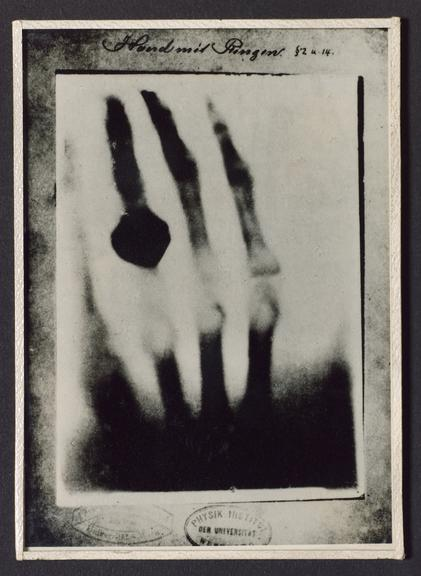
\includegraphics[width=0.725\linewidth]{pics/hand.jpg}

    \column{0.5\textwidth}
    
\includegraphics[width=0.725\linewidth]{pics/Rontgen.jpeg}
  \end{columns}
\end{frame}

\begin{frame}{Applications of X-rays}
Today, Röntgen's X-rays are used in a variety of applications, including Radiotherapy.
\vspace{0.5em}
  \begin{columns}
    \column{0.5\textwidth}
    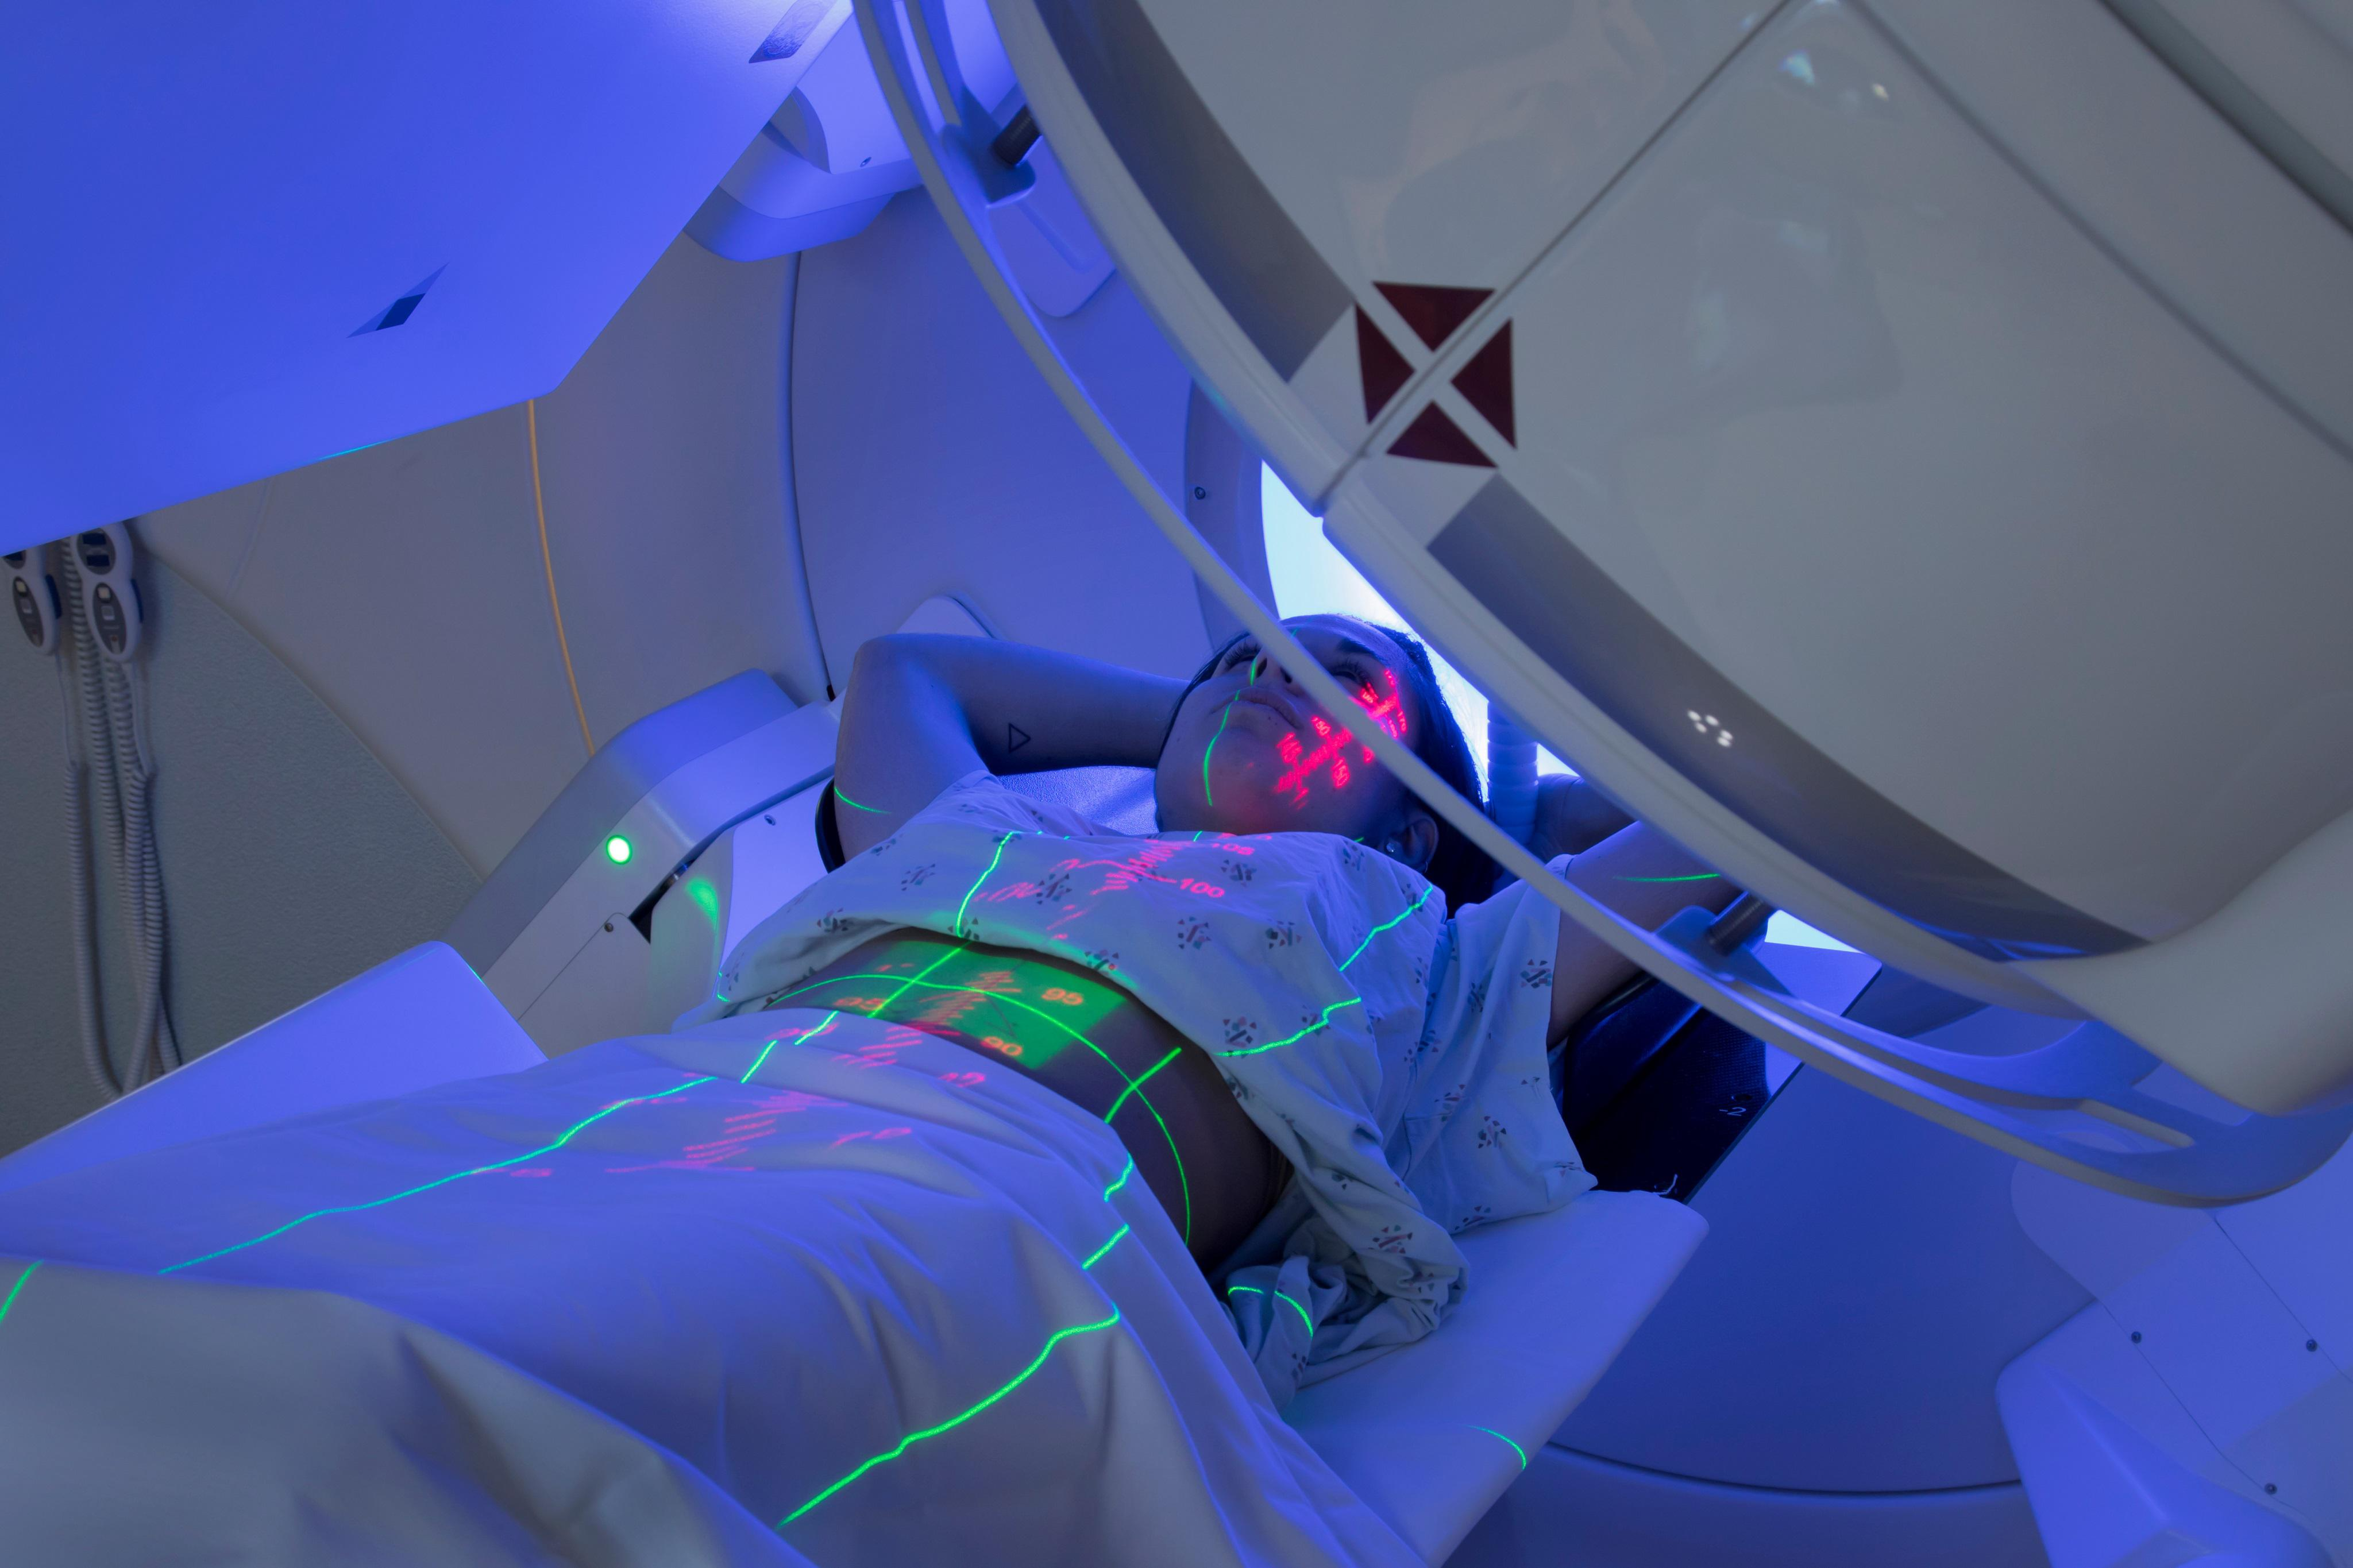
\includegraphics[width=1\linewidth]{pics/RadiationTherapy.jpg}
    \column{0.5\textwidth}
    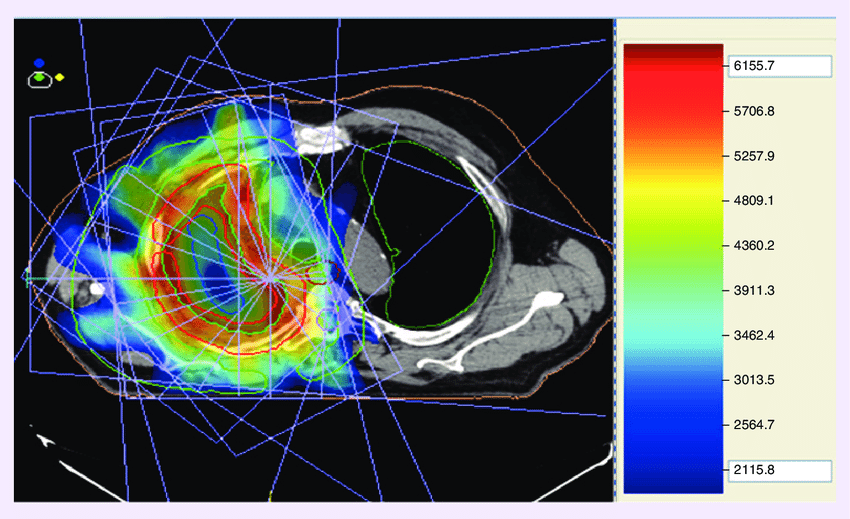
\includegraphics[width=1\linewidth]{pics/RadiationTherapyPlanning.png}
  \end{columns}
\end{frame}

\begin{frame}{Planning a Radiotherapy Treatment}
    \begin{enumerate}
        \setlength{\itemsep}{1em}
        \item We aim to deliver a high radiation dose to the tumor.
        \item We would like to deliver a low radiation dose to healthy tissues.
        \item We want the radiation dose delivered to the tumor to be relatively uniform.
    \end{enumerate}
\end{frame}

\begin{frame}{Optimizing a Radiotherapy Treatment Plan - Notation}
    \begin{enumerate}
        \setlength{\itemsep}{1em}
        \item $[m]$ - the set of all voxel indices.
        \item $T \subseteq [m]$ - the set of all tumor voxels.
        \item $H_k \subseteq [m]$ - the set of all voxels in the $k$-th healthy organ, $\forall\; k \in [K]$.
        \item $n$ - the number of beamlets whose intensity is to be determined.
        \item $\mathbf{D} \in \mathbb{R}^{m \times n}$ - the dose matrix, where $\mathbf{D}_{i,j}$ is the influence the $j$-th beamlet has on the $i$-th voxel.
        \item $N$ - the number of fractions.
        \item $\mathbf{x} \in \mathbb{R}^{N\times n}$ - the intensity of the $n$ beamlets in each of the $N$ fractions.
    \end{enumerate}
    \small{Note: $T\cup\bigcup\limits_{k=1}^K H_k = [m]$}
\end{frame}

\begin{frame}{What's Uncertain?}
    The so-called \textit{physical dose} applied to a voxel $v$ at fraction $f$ is given by:
    \[
    d_{f,v}(\mathbf{x}) = \sum_{i=1}^n \mathbf{D}_{v,i} x_{f,i}
    \]
    where $\mathbf{D}_{v,i}$ is the influence the $i$-th beamlet has on the voxel $v$.

    However, the impact of the \textit{physical dose} also depends on biological factors, such as the oxygenation level of the voxel.

    This information is modeled via a \textit{radiosensitivity vector} $\Phi \in [0,1]^{N\times T}$.

    Accordingly, the \textit{bio-adjusted dose} applied to a voxel $v$ at fraction $f$ is given by:
    \[
    \phi_{f,v} \cdot d_{f,v}(\mathbf{x})
    \]
    Unfortunately, $\Phi$ is estimated from medical images, that are taken days or weeks before the treatment, and so, we only have an uncertain estimate, $\hat{\Phi}$.
\end{frame}

\begin{frame}{Optimizing a Radiotherapy Treatment Plan – Nominal Formulation}
    Taking $\hat{\Phi}$ at face value, we formulate the following LP, which optimizes the radiotherapy treatment plan in accordance with the aforementioned goals:
    \small{
    \begin{align}
        \max_{\mathbf{x} \in \mathbb{R}_+^{N \times n},\; \underline{d} \in \mathbb{R},\; \underline{d}^F \in \mathbb{R}} \quad & \underline{d} + \lambda \underline{d}^F \tag{1.a} \\
        \text{subject to} \quad 
        & \underline{d}^F \le \hat{\phi}_{fv} d_{fv}(\mathbf{x}), && v \in T,\; f \in [N] \tag{1.b} \label{1.b} \\
        & \hat{\phi}_{fv} d_{fv}(\mathbf{x}) \le \mu^F \underline{d}^F, && v \in T,\; f \in [N] \tag{1.c} \label{1.c} \\
        & \underline{d} \le \sum_{f \in [N]} \hat{\phi}_{fv} d_{fv}(\mathbf{x}), && v \in T \tag{1.d} \label{1.d} \\
        & \sum_{f \in [N]} \hat{\phi}_{fv} d_{fv}(\mathbf{x}) \le \mu \underline{d}, && v \in T \tag{1.e} \label{1.e} \\
        & d_{fv}(\mathbf{x}) \le \bar{d}_k^F, && f \in [N],\; k \in [K],\; v \in H_k \tag{1.f} \label{1.f} \\
        & \sum_{f \in [2]} d_{fv}(\mathbf{x}) \le \bar{d}_k, && k \in [K],\; v \in H_k \tag{1.g} \label{1.g}
    \end{align}}
    \vspace{0.5em}
    \begin{center}
    \textit{Nominal Formulation} \quad (\hyperref[1.b]{see constraints 1.b–1.g})
    \end{center}
    \end{frame}

\begin{frame}{Optimizing a Radiotherapy Treatment Plan – Uncertainty Set}
        Here we apply the robust optimization methodology by assuming that the values of $\bm{\Phi}$ are members of the following uncertainty set, henceforth referred to as the \textit{spatially and temporally bound uncertainty set}:
        \vspace{0.5em}
        \small{
        \[
        \stb =
        \left\{
        \bm{\Phi} \in [0, 1]^{N \times |T|} \;\middle|\;
        \begin{array}{ll}
        |\phi_{1v} - \hat{\phi}_{1v}| \leq \delta, & \forall v \in T \\
        |\phi_{fv} - \phi_{fu}| \leq \gamma_{vu}, & \forall f \in [N],\, v, u \in T \\
        |\phi_{fv} - \phi_{(f+1)v}| \leq \sigma, & \forall f \in [N{-}1],\, v \in T
        \end{array}
        \right\}
        \]
        }
    \begin{itemize}
        \item $\delta$ - the maximum allowed deviation from the measured radiosensitivity vector.
        \item $\gamma_{vu}$ - parameters given by a metric-preserving function of the distance between $v$ and $u$. Limits the maximum allowed deviation between the radiosensitivity values of two consecutive fractions.
        \item $\sigma$ - the maximum allowed deviation between the radiosensitivity value of a voxel across two consecutive fractions.
    \end{itemize}
\end{frame}

\begin{frame}{Optimizing a Radiotherapy Treatment Plan – Robust Formulation}
    After a couple of simple algebraic manipulations, we can write the \textit{robust counterpart} of the nominal LP:
    \tiny{
    \begin{align}
        \max_{\mathbf{x} \in \mathbb{R}_+^{N \times n},\; \underline{d} \in \mathbb{R},\; \underline{d}^F \in \mathbb{R}} \quad 
        & \underline{d} + \lambda \underline{d}^F \tag{2.a} \\
        \text{subject to} \quad 
        & \min_{\bm{\Phi} \in \stb} \left\{ \phi_{fv} d_{fv}(\mathbf{x}) \right\} \ge \underline{d}^F, && v \in T,\; f \in [N] \tag{2.b} \label{2.b} \\
        & \max_{\bm{\Phi} \in \stb} \left\{ \phi_{fv} d_{fv}(\mathbf{x}) - \mu \phi_{fu} d_{fu}(\mathbf{x}) \right\} \le 0, && v,u \in T,\; f \in [N] \tag{2.c} \label{2.c} \\
        & \min_{\bm{\Phi} \in \stb} \left\{ \sum_{f \in [N]} \phi_{fv} d_{fv}(\mathbf{x}) \right\} \ge \underline{d}, && v \in T \tag{2.d} \label{2.d} \\
        & \max_{\bm{\Phi} \in \stb} \left\{ \sum_{f \in [N]} \phi_{fv} d_{fv}(\mathbf{x}) - \mu \sum_{f \in [N]} \phi_{fu} d_{fu}(\mathbf{x}) \right\} \le 0, && v,u \in T \tag{2.e} \label{2.e} \\
        & d_{fv}(\mathbf{x}) \le \bar{d}_k^F, && f \in [N],\; k \in [K],\; v \in H_k \tag{2.f} \\
        & \sum_{f \in [2]} d_{fv}(\mathbf{x}) \le \bar{d}_k, && k \in [K],\; v \in H_k \tag{2.g} \label{2.g}
    \end{align}}
\end{frame}

\begin{frame}{Optimizing a Radiotherapy Treatment Plan – Reformulation}
    The robust counterpart is a semi-infinite program — that is, a program with an infinite number of constraints — and must be reformulated to be solvable.
    \small{
    \begin{customlemma}
    Let $\mathcal{U} \subseteq \mathbb{R}^n$ be a Reformulated Robust set. Then for any continuous function $f: \mathbb{R}^{|\mathcal{I}|} \to \mathbb{R}$,
    \[
        \min_{\mathbf{u}_{\mathcal{I}} \in \mathcal{U}} \left\{ f(\mathbf{u}_{\mathcal{I}}) \right\}
        =
        \min_{\mathbf{u}_{\mathcal{I}} \in \mathcal{P}_{\mathcal{I}}(S)} \left\{ f(\mathbf{u}_{\mathcal{I}}) \right\}
    \]
    \end{customlemma}
    \begin{customlemma}
        The projection of $\stb$ onto $\phi_{fv}$ is 
        \[
        P_{{fv}}(\stb) = \left[\min_{\phi_{fv} \in \stb}\{\phi_{fv}\}, \max_{\phi_{fv} \in \stb}\{\phi_{fv}\}\right]
        \quad \forall\; v \in T,\; f \in [2]
        \]
        \end{customlemma}
    }
    \end{frame}

\begin{frame}{Optimizing a Radiotherapy Treatment Plan – 1-D Projections}
    \tiny{
    \begin{customlemma}\label{lem:1-d projection}
        Consider the case where \( N = 2 \), and suppose for any \( u, v \in T \), we have \( \gamma_{uv} = \Gamma(\text{dist}(u, v)) \), where \( \text{dist}(u, v) \) is the voxel-to-voxel distance, and \( \Gamma : \mathbb{R} \to [0, 1] \) is a nondecreasing, subadditive function satisfying \( \Gamma(x) = 0 \iff x = 0 \).
        Define for all \( v \in T \):
        \begin{align}
            \underline{\phi}_{1v}^0 &= \max\left\{ 0,\, \hat{\phi}_{1v} - \delta \right\}, 
            & \quad \bar{\phi}_{1v}^0 &= \min\left\{ \hat{\phi}_{1v} + \delta,\, 1 \right\} \label{phi0} \\[0.8em]
            \underline{\phi}_{1v} &= \max_{u \in T} \left\{ \underline{\phi}_{1u}^0 - \gamma_{uv} \right\},
            & \quad \bar{\phi}_{1v} &= \min_{u \in T} \left\{ \bar{\phi}_{1u}^0 + \gamma_{uv} \right\} \label{phibar} \\[0.8em]
            \underline{\phi}_{2v} &= \max\left\{ 0,\, \underline{\phi}_{1v} - \sigma \right\},
            & \quad \bar{\phi}_{2v} &= \min\left\{ \bar{\phi}_{1v} + \sigma,\, 1 \right\} \label{phiubar}
        \end{align}
        Then,
        \[
        \max_{\phi \in \stb} \phi_{fv} = \bar{\phi}_{fv}, \qquad
        \min_{\phi \in \stb} \phi_{fv} = \underline{\phi}_{fv}
        \]
        \end{customlemma}
    }
\end{frame}

\begin{frame}{Optimizing a Radiotherapy Treatment Plan - Reformulated Constraint \ref{2.b}}
    \begin{corollary}
    Constraint~\ref{2.b} can be rewritten as:
    \[
    \underline{\phi}_{fv} \cdot d_{fv}(\mathbf{x}) \ge \underline{d}^F, \quad v \in T,\; f \in [2] \tag{3.b}
    \]
    \end{corollary}
\end{frame}

\begin{frame}
    {Optimizing a Radiotherapy Treatment Plan - Reformulated Constraint \ref{2.d}}
    \vspace{1em}

    \begin{corollary}
    Constraint~\ref{2.d} can be rewritten as:
    \[
    \sum_{f \in [N]} \underline{\phi}_{fv} \cdot d_{fv}(\mathbf{x}) \ge \underline{d} \tag{3.d}
    \]
    \end{corollary}
\end{frame}

\begin{frame}{Optimizing a Radiotherapy Treatment Plan – 2-D first fraction}
    \tiny{
        \begin{customlemma}
            Suppose \( v \in T \), and let \( \underline{\bm{\phi}} \in \mathbb{R}^{2 \times |T|} \), \( \bar{\bm{\phi}} \in \mathbb{R}^{2 \times |T|} \) have components given by \eqref{phibar} and \eqref{phiubar}, and suppose that for any \( u, v \in T \),
            \[
            \gamma_{uv} = \Gamma\big(\text{dist}(u, v)\big),
            \]
            where \( \text{dist}(u, v) \) is the voxel-wise distance, and \( \Gamma : \mathbb{R} \to [0, 1] \) is a nondecreasing, subadditive function satisfying \( \Gamma(x) = 0 \iff x = 0 \).
            
            Then, the projection of \( \stb \) onto \( (\phi_{1v}, \phi_{1u}) \) satisfies:
            \[
            \mathcal{P}_{1v,1u}(\stb) = \mathcal{U}_{v,u}^{(1)} \equiv 
            \left\{
            \begin{array}{l}
            (\phi_{1v}, \phi_{1u}) \in \mathbb{R}^2 \;\;:\;\;
            \underline{\phi}_{1v} \le \phi_{1v} \le \bar{\phi}_{1v}, \;
            \underline{\phi}_{1u} \le \phi_{1u} \le \bar{\phi}_{1u}, \;
            |\phi_{1v} - \phi_{1u}| \le \gamma_{vu}
            \end{array}
            \right\}
            \]
            \end{customlemma}
    }
\end{frame}

\begin{frame}{Optimizing a Radiotherapy Treatment Plan – 2-D second fraction}
    \tiny{
    \begin{customlemma}
    Suppose \( v \in T \), and let \( \underline{\bm{\phi}} \in \mathbb{R}^{2 \times |T|} \), \( \bar{\bm{\phi}} \in \mathbb{R}^{2 \times |T|} \) have components given by \eqref{phibar} and \eqref{phiubar}. Suppose also that for any \( u, v \in T \),
    \[
    \gamma_{uv} = \Gamma\big(\text{dist}(u, v)\big),
    \]
    where \( \text{dist}(u, v) \) is the distance between voxels \( u \) and \( v \), and \( \Gamma : \mathbb{R} \to [0, 1] \) is a nondecreasing, subadditive function satisfying \( \Gamma(x) = 0 \iff x = 0 \).
    
    Then, the projection of \( \stb \) onto \( (\phi_{2v}, \phi_{2u}) \) is:
    \[
    \mathcal{P}_{2v,2u}(\stb) = \mathcal{U}_{v,u}^{(2)} \equiv 
    \left\{
    \begin{array}{l}
    (\phi_{2v}, \phi_{2u}) \in \mathbb{R}^2 \;\;:\;\;
    \underline{\phi}_{2v} \le \phi_{2v} \le \bar{\phi}_{2v}, \;
    \underline{\phi}_{2u} \le \phi_{2u} \le \bar{\phi}_{2u}, \;
    |\phi_{2v} - \phi_{2u}| \le \gamma_{vu}
    \end{array}
    \right\}
    \]
    \end{customlemma}
    }
    \end{frame}

\begin{frame}
        {Optimizing a Radiotherapy Treatment Plan - Reformulated Constraint \ref{2.c}}
        \vspace{1em}
        \small{
        \begin{customobservation}
        Invoking proposition 7 from \cite{apte2024robust}, we can replace constraint~\ref{2.c} by the constraint pair:
            \begin{align}
            & \bar{\phi}_{fv} \cdot d_{fv}(\mathbf{x}) +
            \max\left\{ \underline{\phi}_{fu},\; \bar{\phi}_{fv} - \gamma_{uv} \right\}
            \cdot (-\mu^F d_{fu}(\mathbf{x}))
            \le 0, \quad v, u \in T,\; f \in [N]
            \tag{$2.\text{c}_1$} \\[0.8em]
            & \max\left\{ \underline{\phi}_{fu} + \gamma_{uv},\; \bar{\phi}_{fv} \right\}
            \cdot d_{fv}(\mathbf{x}) +
            \underline{\phi}_{fu} \cdot (-\mu^F d_{fu}(\mathbf{x}))
            \le 0, \quad v, u \in T,\; f \in [N]
            \tag{$2.\text{c}_2$}
            \end{align}
        \end{customobservation}
        }
\end{frame}

\begin{frame}{Reformulated Robust Optimization Problem (Without commulutive homogeneity)}
    \vspace{-0.5em}
    \tiny{
    \begin{align}
    \max_{\mathbf{x} \in \mathbb{R}_+^{2 \times n},\; \underline{d} \in \mathbb{R},\; \underline{d}^F \in \mathbb{R}} \quad
    & \underline{d} + \lambda \underline{d}^F \tag{3.a} \\
    \text{subject to} \quad
    & \underline{\phi}_{fv} \cdot d_{fv}(\mathbf{x}) \ge \underline{d}^F,
    && v \in T,\; f \in [2] \tag{3.b} \label{3.b} \\[0.5em]
    & \bar{\phi}_{fv} \cdot d_{fv}(\mathbf{x}) +
    \max\left\{ \underline{\phi}_{fu},\; \bar{\phi}_{fv} - \gamma_{uv} \right\}
    \cdot (-\mu^F d_{fu}(\mathbf{x}))
    \le 0,
    && v,u \in T,\; f \in [2] \tag{3.c'} \\[0.5em]
    & \max\left\{ \underline{\phi}_{fu} + \gamma_{uv},\; \bar{\phi}_{fv} \right\}
    \cdot d_{fv}(\mathbf{x}) +
    \underline{\phi}_{fu} \cdot (-\mu^F d_{fu}(\mathbf{x}))
    \le 0,
    && v,u \in T,\; f \in [2] \tag{3.c''} \\[0.5em]
    & \sum_{f \in [2]} \underline{\phi}_{fv} \cdot d_{fv}(\mathbf{x}) \ge \underline{d},
    && v \in T \tag{3.d} \\[0.5em]
    & d_{fv}(\mathbf{x}) \le \bar{d}_k^F,
    && f \in [2],\; k \in [K],\; v \in H_k \tag{3.e} \\[0.5em]
    & \sum_{f \in [2]} d_{fv}(\mathbf{x}) \le \bar{d}_k,
    && k \in [K],\; v \in H_k \tag{3.f}
    \end{align}
    }
    \vspace{0.5em}
    \centering
    \textit{Reformulated Robust Optimization Problem}
    \end{frame}

\section{Numerical Experiments}
\begin{frame}{Numerical Experiments}
    \end{frame}

\section{Future Directions}
\begin{frame}{Future Directions}

\end{frame}
    
    
    
% Bibliography slide
\begin{frame}[allowframebreaks]{References}
  \printbibliography
\end{frame}

\end{document}
